% Options for packages loaded elsewhere
\PassOptionsToPackage{unicode}{hyperref}
\PassOptionsToPackage{hyphens}{url}
%
\documentclass[
]{article}
\usepackage{lmodern}
\usepackage{amsmath}
\usepackage{ifxetex,ifluatex}
\ifnum 0\ifxetex 1\fi\ifluatex 1\fi=0 % if pdftex
  \usepackage[T1]{fontenc}
  \usepackage[utf8]{inputenc}
  \usepackage{textcomp} % provide euro and other symbols
  \usepackage{amssymb}
\else % if luatex or xetex
  \usepackage{unicode-math}
  \defaultfontfeatures{Scale=MatchLowercase}
  \defaultfontfeatures[\rmfamily]{Ligatures=TeX,Scale=1}
\fi
% Use upquote if available, for straight quotes in verbatim environments
\IfFileExists{upquote.sty}{\usepackage{upquote}}{}
\IfFileExists{microtype.sty}{% use microtype if available
  \usepackage[]{microtype}
  \UseMicrotypeSet[protrusion]{basicmath} % disable protrusion for tt fonts
}{}
\makeatletter
\@ifundefined{KOMAClassName}{% if non-KOMA class
  \IfFileExists{parskip.sty}{%
    \usepackage{parskip}
  }{% else
    \setlength{\parindent}{0pt}
    \setlength{\parskip}{6pt plus 2pt minus 1pt}}
}{% if KOMA class
  \KOMAoptions{parskip=half}}
\makeatother
\usepackage{xcolor}
\IfFileExists{xurl.sty}{\usepackage{xurl}}{} % add URL line breaks if available
\IfFileExists{bookmark.sty}{\usepackage{bookmark}}{\usepackage{hyperref}}
\hypersetup{
  pdftitle={Development of an Intended Bifactor Engagement Measure},
  hidelinks,
  pdfcreator={LaTeX via pandoc}}
\urlstyle{same} % disable monospaced font for URLs
\usepackage[margin=1in]{geometry}
\usepackage{graphicx}
\makeatletter
\def\maxwidth{\ifdim\Gin@nat@width>\linewidth\linewidth\else\Gin@nat@width\fi}
\def\maxheight{\ifdim\Gin@nat@height>\textheight\textheight\else\Gin@nat@height\fi}
\makeatother
% Scale images if necessary, so that they will not overflow the page
% margins by default, and it is still possible to overwrite the defaults
% using explicit options in \includegraphics[width, height, ...]{}
\setkeys{Gin}{width=\maxwidth,height=\maxheight,keepaspectratio}
% Set default figure placement to htbp
\makeatletter
\def\fps@figure{htbp}
\makeatother
\setlength{\emergencystretch}{3em} % prevent overfull lines
\providecommand{\tightlist}{%
  \setlength{\itemsep}{0pt}\setlength{\parskip}{0pt}}
\setcounter{secnumdepth}{-\maxdimen} % remove section numbering
\usepackage{booktabs}
\usepackage{longtable}
\usepackage{array}
\usepackage{multirow}
\usepackage{wrapfig}
\usepackage{float}
\usepackage{colortbl}
\usepackage{pdflscape}
\usepackage{tabu}
\usepackage{threeparttable}
\usepackage{threeparttablex}
\usepackage[normalem]{ulem}
\usepackage{makecell}
\usepackage{xcolor}
\ifluatex
  \usepackage{selnolig}  % disable illegal ligatures
\fi
\newlength{\cslhangindent}
\setlength{\cslhangindent}{1.5em}
\newlength{\csllabelwidth}
\setlength{\csllabelwidth}{3em}
\newenvironment{CSLReferences}[2] % #1 hanging-ident, #2 entry spacing
 {% don't indent paragraphs
  \setlength{\parindent}{0pt}
  % turn on hanging indent if param 1 is 1
  \ifodd #1 \everypar{\setlength{\hangindent}{\cslhangindent}}\ignorespaces\fi
  % set entry spacing
  \ifnum #2 > 0
  \setlength{\parskip}{#2\baselineskip}
  \fi
 }%
 {}
\usepackage{calc}
\newcommand{\CSLBlock}[1]{#1\hfill\break}
\newcommand{\CSLLeftMargin}[1]{\parbox[t]{\csllabelwidth}{#1}}
\newcommand{\CSLRightInline}[1]{\parbox[t]{\linewidth - \csllabelwidth}{#1}\break}
\newcommand{\CSLIndent}[1]{\hspace{\cslhangindent}#1}

\title{Development of an Intended Bifactor Engagement Measure}
\author{true \and true \and true \and true}
\date{}

\begin{document}
\maketitle

\hypertarget{introduction}{%
\section{Introduction}\label{introduction}}

In recent years, employee engagement has earned its stripes as a useful
predictor of employee outcomes (Alarcon \& Edwards, 2011; Hanaysha,
2016; Rich et al., 2010). Despite engagement's burgeoning popularity and
emergence into the cultural mainstream, considerable disagreement exists
among psychologists on the definition and factor structure of the
construct.

The ``substantive'' model of engagement describes it in terms of three
dimensions: Vigor, or high levels of energy at work; Dedication, or
feelings of involvement, pride, and meaning in one's work; and
Absorption, or concentration and flow while working (Schaufeli et al.,
2002). On the other hand, the now-resurgent tripartite model of
attitudes divides attitudes into conitive, affective, and behavioral
components (Rosenberg, 1960).

Breaking from the traditional scale development approach, in which each
item only indicates one construct, we sought to develop an engagement
measure in which each item simultaneously captures a dimension from
\emph{both} the substantive and attitudinal models. In so doing, we aim
to construct a scale with very broad content domain coverage relative to
its length.

\hypertarget{methods}{%
\section{Methods}\label{methods}}

50 items were generated to semantically reflect one dimension each from
the substantive and attitudinal models. For example, ``I speak
positively about this organization to others'' indicates both the
dedication and behavioral dimensions from the substantive and
attitudinal models respectively. Graduate students and faculty sorted
each item twice to their corresponding dimension within the substantive
and attitudinal models. The 36 items that were most consistently sorted
were retained for the study. 330 working adult participants were
gathered via snowball sampling and responded to this set of items.

\hypertarget{item-reduction}{%
\subsection{Item Reduction}\label{item-reduction}}

Our team used two parallel scale development methods: one focusing on
corrected item-total correlations, the other focusing on CFA
modification indices. In the former approach, the item with the lowest
corrected item-total correlation was removed from the scale definition.
This process was iterated after each item deletion until only two items
per each of the nine pairs of substantive and attitudinal dimensions
remained.

The CFA modification index approach focused on item retention rather
than deletion. We ran two parallel CFAs, one on the substantive model
and the other on the attitudinal model. We prioritized the alternative
model predicted model associations as items to retain.

The parallel item reduction approaches yielded two very similar, yet
distinct, 18-item scale definitions. We merged these scales into a final
20-item scale definition based on wording preference and maximizing
content domain coverage.

\begin{figure}

{\centering 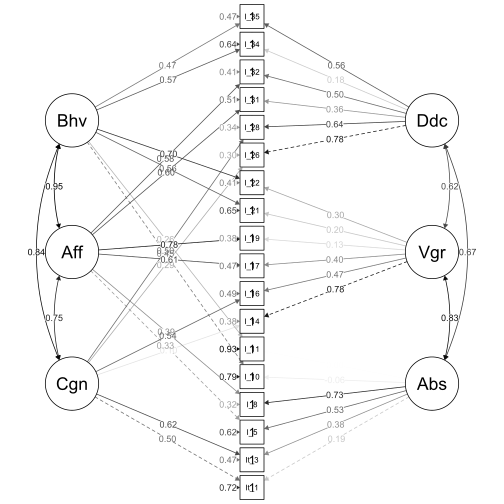
\includegraphics[width=0.8\linewidth]{bifactorplot} 

}

\caption{Bifactor structure}\label{fig:bifactorplot}
\end{figure}

Final 20-item scale definition

Substantive

Attitudinal

Corrected item-total correlation

Absorption

Cognitive

I am able to concentrate on my work without getting distracted

Absorption

Cognitive

I find it difficult to mentally disconnect from work

Absorption

Cognitive

Time passes quickly while I'm working

Absorption

Affective

I enjoy thinking about work even when I'm not at work

Absorption

Affective

I love starting my workday

Absorption

Behavioral

I have to be reminded to take breaks while I'm at work

Absorption

Behavioral

I never miss a work deadline

Vigor

Cognitive

Thinking about work saps my energy

Vigor

Cognitive

I'm able to maintain good levels of energy throughout the workday

Vigor

Affective

I enjoy spending time completing my job tasks

Vigor

Affective

I feel motivated to go beyond what is asked of me at work

Vigor

Behavioral

When work is slow I find ways to be productive

Vigor

Behavioral

I express enthusiasm for my job while at work

Dedication

Cognitive

I believe this company cares about my career goals

Dedication

Cognitive

I plan to stay with this company as my career advances

Dedication

Cognitive

This organization challenges me to work at my full potential

Dedication

Affective

I feel proud of my accomplishments within this organization

Dedication

Affective

My job makes me feel like I'm part of something meaningful

Dedication

Behavioral

I embrace challenging situations at work

Dedication

Behavioral

I speak positively about this organization to others

\hypertarget{results}{%
\section{Results}\label{results}}

Table @ref(tab:items) shows the final set of 20 items. All data analysis
was conducting in R 4.1.0 using the packages \texttt{tidyverse} (Wickham
et al., 2019), \texttt{DT} (Xie et al., 2021), \texttt{lavaan} (Rosseel,
2012), \texttt{semPlot} (Epskamp, 2019), \texttt{psych} (Revelle, 2021)
and \texttt{posterdown} (Thorne, 2022).

Coefficient alphas for subscales ranged from 0.69 for absorption to 0.86
for affective. The bifactor model with Full Information Maximum
Likelihood estimation displayed strong fit, \(\chi^2\)(111, N = 282) =
264.70, \emph{p} \textless{} .001, CFI = 0.92, AIC = 14113.31, RMSEA =
0.07.

Figure @ref(fig:bifactorplot) shows the factor loadings of each item on
its respective substantive and attitudinal dimensions. Figure
@ref(fig:corrplot) shows subscale-level intercorrelations. Note that
correlations between subscales inheriting from different models (e.g.,
cognitive and vigor) are artificially inflated due to one third of items
being shared. Correlations \emph{within} models are uninflated.

\begin{figure}

{\centering 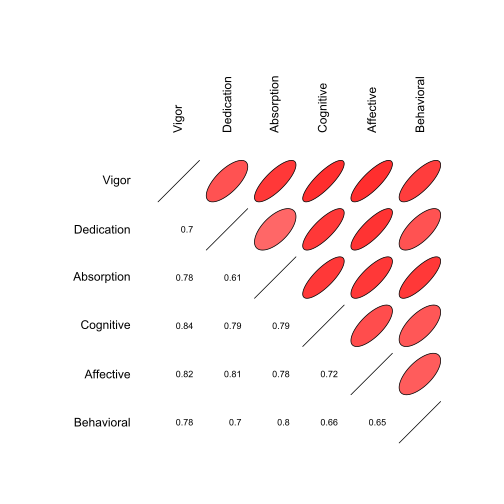
\includegraphics[width=0.8\linewidth]{corrplot} 

}

\caption{Correlations among subscales}\label{fig:corrplot}
\end{figure}

\hypertarget{discussion}{%
\section{Discussion}\label{discussion}}

The present research introduces a novel measure of engagement, developed
in English and available for free. By designing items to correspond to
two separate factor structures, we effectively double our content domain
coverage with the same number of items. A convergent and discriminant
validation study is currently underway, which is also intended to
further reduce the scale definition to 18 items. Most novelly, we
intentionally embrace complexity in scale development. We believe this
approach has promising implications for developing measures which
reconcile, rather than reject, disparate models of constructs. It it our
hope that future researchers will weigh the benefits of broadening item
complexity against the understandable desire for parsimony.

\begingroup
\setlength{\parindent}{-0.5in}
\setlength{\leftskip}{0.5in}

\hypertarget{refs}{}
\begin{CSLReferences}{0}{0}
\end{CSLReferences}

\end{document}
